%%%%%%%%%%%%%%%%%%%%%%%%%%%%%%%%%%%%%%%%%
% a0poster Landscape Poster
% LaTeX Template
% Version 1.0 (22/06/13)
%
% The a0poster class was created by:
% Gerlinde Kettl and Matthias Weiser (tex@kettl.de)
% 
% This template has been downloaded from:
% http://www.LaTeXTemplates.com
%
% License:
% CC BY-NC-SA 3.0 (http://creativecommons.org/licenses/by-nc-sa/3.0/)
%
%%%%%%%%%%%%%%%%%%%%%%%%%%%%%%%%%%%%%%%%%

%----------------------------------------------------------------------------------------
%	PACKAGES AND OTHER DOCUMENT CONFIGURATIONS
%----------------------------------------------------------------------------------------

\documentclass[a0,landscape]{a0poster}

\usepackage{multicol} % This is so we can have multiple columns of text side-by-side
\columnsep=50pt % This is the amount of white space between the columns in the poster
\columnseprule=3pt % This is the thickness of the black line between the columns in the poster

\usepackage[svgnames]{xcolor} % Specify colors by their 'svgnames', for a full list of all colors available see here: http://www.latextemplates.com/svgnames-colors

\usepackage{times} % Use the times font
%\usepackage{palatino} % Uncomment to use the Palatino font

\usepackage{graphicx} % Required for including images
\graphicspath{{figures/}} % Location of the graphics files
\usepackage{booktabs} % Top and bottom rules for table
\usepackage[font=small,labelfont=bf]{caption} % Required for specifying captions to tables and figures
\usepackage{amsfonts, amsmath, amsthm, amssymb} % For math fonts, symbols and environments
\usepackage{wrapfig} % Allows wrapping text around tables and figures
\usepackage[
    backend=biber, 
    style=numeric, 
    sorting=none, 
    maxbibnames=1,    % Affiche seulement le 1er auteur suivi de "et al."
    doi=false,        % Supprime le DOI
    isbn=false,       % Supprime l'ISBN
    url=false,        % Supprime les liens URL
    eprint=false      % Supprime les liens Arxiv
    ]{biblatex}       % Use biblatex 
\addbibresource{sample.bib}

% Use only necessary fields
\AtEveryBibitem{
    \clearfield{abstract}
    \clearfield{note}
    \clearfield{pages}
    \clearfield{series}
}

\begin{document}

%----------------------------------------------------------------------------------------
%	POSTER HEADER 
%----------------------------------------------------------------------------------------

% The header is divided into three boxes:
% The first is 55% wide and houses the title, subtitle, names and university/organization
% The second is 25% wide and houses contact information
% The third is 19% wide and houses a logo for your university/organization or a photo of you
% The widths of these boxes can be easily edited to accommodate your content as you see fit

\begin{minipage}[b]{0.55\linewidth}
    \veryHuge \color{NavyBlue} \textbf{Explaining a classifier's decisions} \color{Black} \\ \vspace{1cm} % Title

    \huge \textbf{Noé Mastrorillo \& Axel Pigeon \& Antoine Sinatti \& Matthias Tortosa} \\ % Author(s)
    \huge  University of Toulouse, France \\
\end{minipage}
%
\begin{minipage}[b]{0.25\linewidth}
    \color{DarkSlateGray}\Large \textbf{Contact Information:}\\
    \texttt{noe.mastrorillo@utoulouse.fr}\\
    \texttt{axel.pigeon@utoulouse.fr}\\
    \texttt{antoine.sinatti@utoulouse.fr}\\
    \texttt{matthias.tortosa@utoulouse.fr}\\
\end{minipage}
%
\begin{minipage}[b]{0.19\linewidth}
    
\includegraphics[width=12cm]{logo.png} % Logo or a photo of you, adjust its dimensions here
\end{minipage}

\vspace{1cm} % A bit of extra whitespace between the header and poster content

%----------------------------------------------------------------------------------------

\begin{multicols}{4} % This is how many columns your poster will be broken into, a poster with many figures may benefit from less columns whereas a text-heavy poster benefits from more

%----------------------------------------------------------------------------------------
%	ABSTRACT
%----------------------------------------------------------------------------------------

\color{Navy} % Navy color for the abstract

\begin{abstract}

Sed fringilla tempus hendrerit. Vestibulum ante ipsum primis in faucibus orci luctus et ultrices posuere cubilia Curae; Etiam ut elit sit amet metus lobortis consequat sit amet in libero. Lorem ipsum dolor sit amet, consectetur adipiscing elit. Phasellus vel sem magna. Nunc at convallis urna. isus ante. Pellentesque condimentum dui. Etiam sagittis purus non tellus tempor volutpat. Donec et dui non massa tristique adipiscing. Quisque vestibulum eros eu. Phasellus imperdiet, tortor vitae congue bibendum, felis enim sagittis lorem, et volutpat ante orci sagittis mi. Morbi rutrum laoreet semper. Morbi accumsan enim nec tortor consectetur non commodo nisi sollicitudin. Proin sollicitudin. Pellentesque eget orci eros. Fusce ultricies, tellus et pellentesque fringilla, ante massa luctus libero, quis tristique purus urna nec nibh.

\end{abstract}

%----------------------------------------------------------------------------------------
%	INTRODUCTION
%----------------------------------------------------------------------------------------

\color{SaddleBrown} % SaddleBrown color for the introduction

\section*{Introduction}

%----------------------------------------------------------------------------------------
%	SHAP 
%----------------------------------------------------------------------------------------


\color{DarkSlateGray} % DarkSlateGray color for the rest of the content

\section*{Shapley values based XAI}

\newcommand{\mS}{\mathcal{S}}
\newcommand{\mF}{\mathcal{F}}
\newcommand{\mP}{\mathcal{P}}
\newcommand{\mD}{\mathcal{D}}
\newcommand{\mbF}{\mathbb{F}}
\newcommand{\mbE}{\mathbb{E}}

In this section, we present local explanation methods based on the Shapley values concept from game theory that give an importance score to each feature in the prediction of a single instance. Shapley values provide a mathematically fair and unique method to attribute the payoff of a cooperative game to the players. Formally, we define the coalitional game $(\mF, v)$ composed of the set of the $n$ numbered features used in the prediction $\mF = \{1, \dots, n\}$ and the evaluation function $v(\mS) = \mbE[f(X) | X_{\mS} = x_{\mS}]$ for all sub-coalition $\mS \subset \mF$, where $f$ is the classification function representing our model and $x_\mS = y_\mS$ means that instances $x$ and $y$ share the same values for the features in $\mS$. The Shapley value for a feature $i \in \mF$ is defined as follows:

\begin{equation}
    \phi_i = \frac{1}{n} \sum_{\mS \in \mF\backslash\{i\}} \binom{n-1}{|\mS|}^{-1} \bigl( \mbE[f(X) | X_{\mS\backslash\{i\}} = x_{\mS\backslash\{i\}}] - \mbE[f(X) | X_{\mS} = x_{\mS}] \bigr)
\end{equation}

We see that the Shapley value of a feature $i$ is computed by going through all the coalitions not containing $i$ and looking at the payoff difference with and without the feature $i$ involved.

From the efficiency axiom of the Shapley values, we get the following property:

\begin{equation}
    \sum_{i \in \mF} \phi_i(v) = \mbE[f(X) | X_{\mF} = x_{\mF}] - \mbE[f(X) | X_{\emptyset} = x_{\emptyset}] = f(x) - \mbE[f(X)]
\end{equation}

Therefore, the sum of the importance is equal to the actual predicted value minus a reference contribution that is the mean of all the predictions for the distribution on the input $X$.

Figure \ref{fig:shap-titanic} vizualises computed importance scores for the prediction of a naive Bayes classifier on an instance of the Titanic dataset.

\begin{center}
    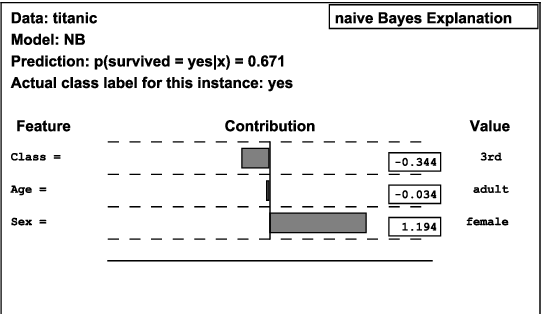
\includegraphics[width=0.8\linewidth]{shap_titanic.png}
    \captionof{figure}{Feature importance attributions computed with Shapley values for the decision of a naive Bayes model on an instance of the Titanic dataset}
    \label{fig:shap-titanic}
\end{center}

\subsection*{Approximation}

The computation of exact Shapley values is intractable as it requires to explore all the sub-coalitions which are in exponential number. Moreover, the computation of the evaluation function requires to explore all the input space. Previous work have come up with sampling methods to get an approximation in polynomial time. Sub-coalitions are sampled by taking all the features preceiding $i$ in random orderings $O_j$ of $\mF$: $\mS_j = Pre_i(O_j)$. The reference instances $X$ are sampled following the distribution of input instances.


%----------------------------------------------------------------------------------------
%	CONCLUSIONS
%----------------------------------------------------------------------------------------

\section*{Perturbation model-agnostic method}

Perturbation methods identify which input features most significantly influence a 
black-box model's decision process. These model-agnostic techniques compare the model's 
output for an original instance against its predictions for perturbed samples. By observing 
how these modifications affect the classification, we can quantify the importance of each 
feature without accessing the model's internal architecture.

\subsection*{LIME}

LIME (Local Interpretable Model-Agnostic Explainer) generates local surrogates to approximate a 
black-box model $f$ \cite{ribeiro_why_2016}. 

\textbf{Key Principle}: It minimizes a loss function $\mathcal{L}(f,g,\pi_x)$ to ensure local fidelity
while keeping the explanation model $g$ simple enough ($\Omega(g)$) for humans.

\textbf{Limitation}: The explanation depends heavily on the kernel width $\pi_x$ and sampling, leading 
to potential instability. 

A most global explanation of the black-box model can be provided by SP-LIME which 
select a set of local and non-redundant LIME explanations. 

\begin{center}
    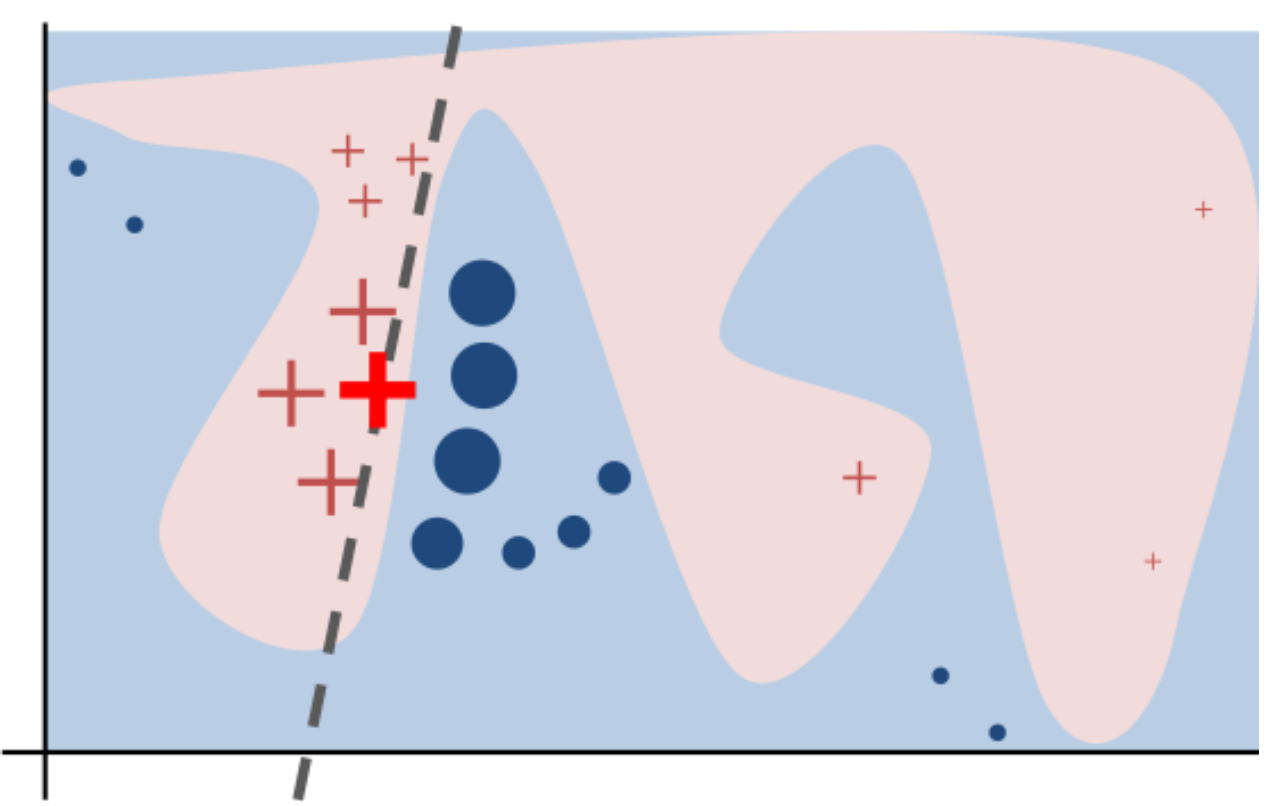
\includegraphics[width=0.8\linewidth]{LIME_schema.png}
    \captionof{figure}{LIME linear local approximation. 
        Black-box model $f$ classes is represented in blue/gray. The red 
        cross represents an explained instance and the others 
        symbols are the perturbation samples generated from the original. 
        The dotted line represents the local approximation of $g$.}
    \label{fig:LIME_graph}
\end{center}

\subsection*{Anchors}

Anchors were developed to solve the lack of clear boundaries provided by LIME. 
To perform that, Anchors generates IF-THEN rules which 'anchor' a prediction. 
This set of short and disjoint rules are more comprehensible and then preferred by 
the users \cite{ribeiro_anchors_2018}.

\textbf{Formal Definition}: A rule $A$ is an Anchor for $x$ if $A(x)=1$ and it maintains high precision $\tau$ among its neighbors:
\begin{equation}
    \mathbb{E}_{\mathcal{D}(z \mid A)}[1_{f(x)=f(z)}] \geqslant \tau
\end{equation}
with $ \mathcal{D}(x \mid A)$ the distribution of neighbors of $x$ wich satisfy the Anchor $A$. 

% Formally, Anchors are built on a set of predicates $\{a_i\}$ called a "rules". We can 
% also see it as a function of instances $x \in X$ :
% $$ A : 
%     \begin{cases}
%         X \longrightarrow \{0, 1\} \\ 
%         x \longmapsto 
%         \begin{cases}
%             1 \text{ if all rules are true for } x \\
%             0 \text{ otherwise}
%         \end{cases}
%     \end{cases}
% $$
% to link a set of rules $A$ on a prediction $f(x)$ (where $f : X \longrightarrow Y$ 
% is the black-box model). Finally, $A$ is an Anchor of $x$ if $A(x) = 1$ 
% and $A$ is a sufficient condition for the prediction $y = f(x)$ :
%     \begin{equation}
%         \mathbb{E}_{\mathcal{D}(z \mid A)}[1_{f(x)=f(z)}] \geqslant \tau
%     \end{equation}
% with $\tau$ the desired level of precision of the Anchor on $x$ \cite{ribeiro_anchors_2018}.
% Here, $ \mathcal{D}(x \mid A)$ represents the distribution of neighbors of $x$ 
% which satisfy the Anchor $A$. 

% Because the number of all possible Anchor is exponential, we cannot perform an 
% exhaustive search. That's why the article introduced the Bottom-Up approach:
% \begin{enumerate}
%     \item \emph{Initialization}: The anchor $A$ is initialized as an empty rule (applying to all instances).
%     \item \emph{Candidate Generation}: In each iteration, a set of candidate rules $\mathcal{A}$ is generated by extending $A$ with one additional feature predicate $\{a_i\}$: $\mathcal{A} = \{A \wedge a_i, A \wedge a_{i+1}, A \wedge a_{i+2}, ...\}$
%     \item \emph{Selection via Multi-Armed Bandit (MAB)}: To identify the best 
%     candidate without an exhaustive number of calls to $f$, the problem is 
%     formulated as a pure-exploration multi-armed bandit problem. The \emph{KL-LUCB} 
%     algorithm is used to find the rule with the highest precision using a minimal 
%     set of samples \cite{ribeiro_anchors_2018}.
%     \item \emph{Termination}: The process terminates when a rule meets the statistical precision constraint: $\mathbb{P} (prec(A) \geqslant \tau) \geqslant 1 - \delta$.
% \end{enumerate}

Computing Anchors is a combinatorial optimization problem. To handle the exponential search space, a 
\textbf{Bottom-Up approach} is used:
\begin{itemize}
    \item \textbf{Candidate Generation}: Rules are extended iteratively with additional predicates.
    \item \textbf{Selection via MAB}: A Multi-Armed Bandit (\textit{KL-LUCB}) algorithm identifies 
    the most precise candidates using minimal model calls \cite{ribeiro_anchors_2018}.
    \item \textbf{Beam Search}: To avoid purely greedy results, the algorithm maintains $B$ candidates, 
    finally outputting the one with the \textbf{highest coverage}: $cov(A) = \mathbb{E}_{\mathcal{D}(z)} [A(z)]$.
\end{itemize}

%----------------------------------------------------------------------------------------
%	CONCLUSIONS
%----------------------------------------------------------------------------------------

\color{SaddleBrown} % SaddleBrown color for the conclusions to make them stand out

\section*{Conclusions}

\begin{itemize}
\item Pellentesque eget orci eros. Fusce ultricies, tellus et pellentesque fringilla, ante massa luctus libero, quis tristique purus urna nec nibh. Phasellus fermentum rutrum elementum. Nam quis justo lectus.
\item Vestibulum sem ante, hendrerit a gravida ac, blandit quis magna.
\item Donec sem metus, facilisis at condimentum eget, vehicula ut massa. Morbi consequat, diam sed convallis tincidunt, arcu nunc.
\item Nunc at convallis urna. isus ante. Pellentesque condimentum dui. Etiam sagittis purus non tellus tempor volutpat. Donec et dui non massa tristique adipiscing.
\end{itemize}

\color{DarkSlateGray} % Set the color back to DarkSlateGray for the rest of the content

%----------------------------------------------------------------------------------------
%	FORTHCOMING RESEARCH
%----------------------------------------------------------------------------------------

% \section*{Forthcoming Research}

% Vivamus molestie, risus tempor vehicula mattis, libero arcu volutpat purus, sed blandit sem nibh eget turpis. Maecenas rutrum dui blandit lorem vulputate gravida. Praesent venenatis mi vel lorem tempor at varius diam sagittis. Nam eu leo id turpis interdum luctus a sed augue. Nam tellus.

 %----------------------------------------------------------------------------------------
%	REFERENCES
%----------------------------------------------------------------------------------------

\printbibliography

%----------------------------------------------------------------------------------------
%	ACKNOWLEDGEMENTS
%----------------------------------------------------------------------------------------

% \section*{Acknowledgements}

% Etiam fermentum, arcu ut gravida fringilla, dolor arcu laoreet justo, ut imperdiet urna arcu a arcu. Donec nec ante a dui tempus consectetur. Cras nisi turpis, dapibus sit amet mattis sed, laoreet.

%----------------------------------------------------------------------------------------

\end{multicols}
\end{document}